\epigraph{\textit{Logic is the foundation of the certainty of all the Knowledge we acquire.}}{-- \textup{Leonhard Euler}}

As we have seen thus far, the thesis' main goal is to create a tool capable of creating subsets out of a Knowledge Graph provided a \texttt{Shape Expression} schema. To achieve so, in this chapter, we will explore two main ideas. Firstly, we will comment on the possibility of implementing the Pregel framework in Rust. Secondly, we will design a tool for validating a Knowledge Graph against a \texttt{Shape Expression}, following a novel approach.

\section{Pregel-rs}

The \texttt{pregel-rs} library is a Rust fork of the original Pregel framework that we have already discussed in chapter \ref{chapter:theory}. This library is available on GitHub\footnote{\url{https://github.com/angelip2303/pregel-rs}}.

\subsection{Design}

Long has been discussed about the Pregel framework, thus far. However, for us to implement it, we need to make certain design decisions. This section will outline the compromises we have made to successfully implement it in Rust.

First and foremost, it should be acknowledged that when transitioning from the Scala-based solution to the Rust-based one, we were fully aware that building the solution on top of existing projects would not be feasible. Rust, being a relatively new language, is not as mature as Java. Consequently, certain features would need to be developed from scratch. Thus, we started the development of the Pregel library, which will be utilized to implement the subgraph matching algorithm.

It is important to note that we have deliberately separated the framework from the algorithm implementation addressed in this thesis. This decision was made to maximize the framework's flexibility. By adopting this approach, not only can we utilize the framework in other projects, but we can also extend its capabilities to support additional features. To put an example, we have successfully incorporated the \textit{PageRank} algorithm into the framework as an additional feature to demonstrate its versatility. In the following sections, we will discuss the design and implementation details of the Pregel library.

\label{section:pregel-rs}
\subsubsection{The \texttt{pregel-rs} library}

Recall that Rust is heavily oriented to be executed in single machines. This means that we won't use the Pregel framework to process graphs in a distributed manner. Instead, we will use it to process graphs in a \textit{centralized system}. Back when the Pregel framework was introduced, the hardware resources available for single-node systems were limited. However, nowadays, we can leverage the benefits of multi-core processors to process graphs in a centralized manner. Thus we will make use of techniques such as \textit{multi-threading} to process graphs in a single machine. Note that the creation of the \texttt{wd2duckdb} tool was motivated by the idea of trying to make it fit the whole graph in memory. To put it into perspective, as of 2023, we, as customers, can purchase a memory module with a capacity of 128 GB with a total cost of $\$269.90$. However, this was not the case back in 2010, when the Pregel framework was introduced. Thus, we are hopeful that we can create a Pregel-like framework that instead of processing graphs in a distributed manner, can make use of the hardware resources available in a single machine; this is, a \textit{multi-threaded Pregel}. Recall what we have mentioned in section \ref{section:rust} about the way \textit{concurrency and parallelism} are implemented in Rust.

The idea then is to optimize the use of memory as much as we can to process graphs in a single machine. As a comparison, the size of the Wikidata JSON dump created as of August the $21^{th}$ 2017 is 16.94 GB compressed (224.42 GB uncompressed), while the \texttt{.duckdb} database file created by the \texttt{wd2duckdb} tool is 9.38 GB. This means that we can fit the whole graph in memory, and hence, we can fit the graph in a single machine. However, we need to be careful when processing the graph, as we can easily run out of memory by annotating it with additional information. To avoid this, we will make use of the \textit{lazy evaluation} technique. This mechanism will allow us to process the graph in a \textit{streaming} manner, which will reduce the memory footprint of the application. More into this will be discussed later on.

Firstly, we are describing the series of steps that the Pregel framework follows to process a graph. This sequence is depicted in figure \ref{fig:sequence}. The execution starts by sending the initial messages to the vertices at iteration 0. Then, the first -- actual -- \textit{superstep} begins. This loop will last until the current iteration is greater than the threshold set at the creation of the Pregel instance. At each iteration, the vertices will send messages to their neighbors, provided the given direction, and subsequently, they may receive messages sent from other nodes. Moving forward, an aggregation function is applied, and the vertices are updated accordingly. Finally, the iteration counter is incremented, and the next iteration starts until the threshold is reached.

\begin{figure}[ht]
    \centering
    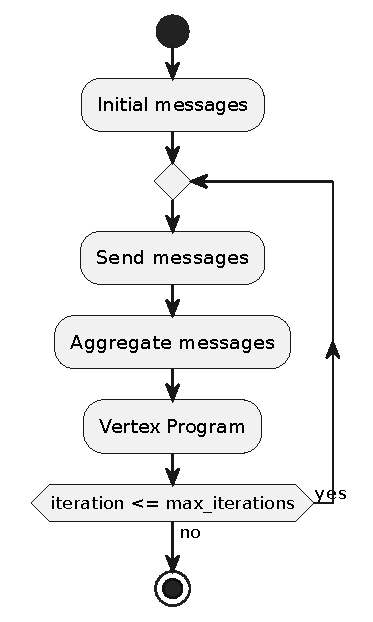
\includegraphics[width=0.4\textwidth]{diagrams/11-1_pregel.pdf}
    \caption{The Pregel framework as implemented in \texttt{pregel-rs}}
    \label{fig:sequence}
\end{figure}

As you can observe, the described process is far from being complex. Thus, we can agree that the Pregel framework is a simple abstraction for graph processing. However, this simplicity is what makes the Pregel paradigm so powerful. By abstracting the underlying model, we can focus on the problem at hand, rather than the implementation details of the framework. By doing so, we can focus on the implementation of the \textit{subgraph matching algorithm}, rather than the implementation details of the Pregel model itself. Now that we have a better understanding of what we are trying to build, we can move forward and discuss some of the design decisions we have made.

\subsubsection{The Builder pattern}

In Rust, there is no direct support for constructors. Instead, the convention is to use an associated function called \texttt{new} that returns an instance of the \texttt{struct}. However, this restricts the creation of objects to only one possible representation, since multiple functions cannot have the same identifier. Unlike Java, where we can have multiple constructors with the same name, as long as they have different parameters. To overcome this limitation and enable the creation of different representations of the same object, we can use the \textit{Builder pattern}.

\begin{figure}[ht]
    \centering
    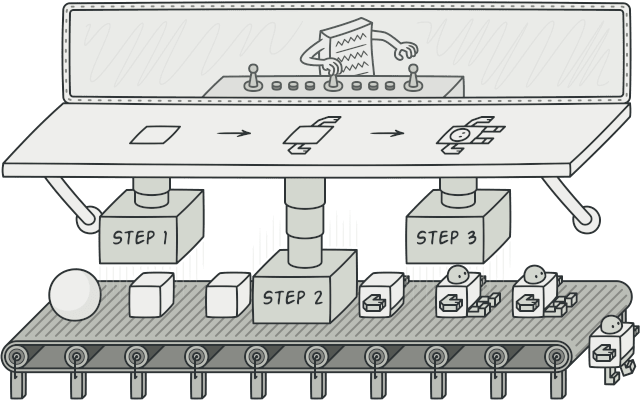
\includegraphics[width=0.66\textwidth]{diagrams/11-2_builder.png}
    \caption[Diagram showing the idea behind the \textit{Builder pattern}]{Diagram showing the idea behind the \textit{Builder pattern}\footnotemark}
\end{figure}
\footnotetext{\url{https://refactoring.guru/design-patterns/builder}}

This is a creational design pattern that allows us to decouple the construction of a complex object from its functionality. By separating the construction process, we gain the flexibility to create diverse representations of the object itself. This pattern effectively resolves the issue of dealing with constructors that have an excessive number of parameters and also addresses Rust's limitation of having only one \texttt{new} function per \texttt{struct}. It also allows us to \textit{create} objects in a -- somewhat -- functional manner, which is a common practice in Rust. As a last remark, the \textit{Builder pattern} allows us to create a default representation of the object, which is useful when we want to create a default configuration of it, and then modify it accordingly. What's more, it allows us to build objects in such a manner that some configuration aspects are optional. In the example below we can observe the creation of a Pregel instance using the Builder pattern. What we are doing is creating a default configuration of the Pregel instance, by calling the \textit{new} function, passing the \texttt{GraphFrame} object, which is the only required parameter. Then, by subsequent calls to the builder methods we can modify the object's representation. As an example, we are setting the maximum number of iterations to 4. Finally, we are calling the \texttt{build} function which will return the -- actual -- Pregel instance with the desired representation. Note that, in this case, what we are building is the so-called \textit{PageRank} algorithm\footnote{\url{https://github.com/angelip2303/pregel-rs/blob/main/examples/pagerank.rs}}, which is a well-known algorithm for ranking web pages.

\begin{code}[Creating a Pregel instance using the Builder pattern]
    \inputminted{rust}{code/listings/11-3_pagerank.rs}
\end{code}

\vspace*{1em}

\subsection{Implementation}

We will now discuss the implementation details of the Pregel library that we have just described. Recall that we are willing to create a tool that is implemented on top of a DataFrame API, as we want to leverage the benefits of this abstraction that we have already discussed in chapter \ref{chapter:refactoring}. Thus, we will now comment on the implementation details of the Pregel library.

\subsubsection{The \texttt{GraphFrame} struct}

The first step is to create a representation of the graph that we are going to process. To do so, we have created the \texttt{GraphFrame} struct. This struct is a wrapper around the \texttt{pola-rs} \texttt{DataFrame} library, which is the equivalent in Rust to Apache Spark's \texttt{DataFrame API}, as we have seen in chapter \ref{chapter:analysis}. This \texttt{struct} is responsible for storing the graph's vertices and edges, as well as extending its basic functionality to support some useful operations. For example, we have implemented the \texttt{from\_edges} function, which is responsible for creating a \texttt{GraphFrame} instance from a set of edges. This function is useful since it allows us the creation of the \texttt{GraphFrame} from the entities that we have extracted from the Wikidata JSON dump in chapter \ref{chapter:wd2duckdb}.

As we have introduced in section \ref{section:pregel-rs}, the way we are implementing the \texttt{pregel-rs} library is through a \texttt{Lazy API}\footnote{\url{https://pola-rs.github.io/polars-book/user-guide/concepts/lazy-vs-eager/}}. What we mean by this is that operations are not computed until we explicitly specify so. This has a great advantage when working with large datasets, as we can \textit{optimize} the query we are building. Let me clarify this. When we evaluate functions more traditionally; that is, \textit{eager evaluation}, expressions are computed as soon as they are defined. This means that, if we have a chain of operations, each operation will be computed as they appear in the code. However, things are different when using \textit{lazy evaluation}, as expressions are not computed until we need the actual result of the evaluation. This allows \textit{query engines} to optimize\footnote{\url{https://pola-rs.github.io/polars-book/user-guide/lazy/optimizations/}} the query, by reordering the operations in such a way that the number of actual computations is reduced. In the example below, we can observe how operations are not computed until we call the \texttt{collect} function, in line 20, which is the one that triggers the computation. Note that we can use this technique as we call the \texttt{lazy} function before referring to the computations we want to perform over the dataset. This has another enormous advantage, which is that we can \texttt{clone} the objects that we are working with, without having to worry about the performance implications of doing so. This is because, as we have mentioned, the actual computation is not yet performed, and hence, we are just \texttt{cloning} the \textit{query plan}\footnote{\url{https://stackoverflow.com/questions/72320911/how-to-avoid-deep-copy-when-using-groupby-in-polars-rust}}.

\begin{code}[GraphFrame implementation in \texttt{pregel-rs}]
    \inputminted{rust}{code/listings/11-1_graph.rs}
\end{code}

\vspace*{1em}

\subsubsection{The \texttt{Pregel} framework}

Thus far, quite a lot has been said about different \texttt{structs} and features that are helpful for the implementation of the Pregel algorithm. However, we have not yet discussed the actual algorithm. In this section, we will comment on the implementation details of the Pregel model in Rust, which is the core of the \texttt{pregel-rs} library. Recall diagram \ref{fig:sequence} where we showed the different steps that are involved in the Pregel framework.

First, we will start by describing the \texttt{initial\_message} step\footnote{\url{https://github.com/angelip2303/pregel-rs/blob/main/src/pregel.rs\#L764}}. Note that, at this point, we are working with a Graph containing a bunch of vertices and edges. No operation has been performed yet. Thus, we need to create -- at least -- one extra column for the messages to be sent, back and forth. What's more, we have to initialize that column to a certain value, which is specified by the user during the configuration of the Pregel instance. Regarding the point in time at which we \texttt{collect} the results of the computation, this will be performed at the end of each \textit{superstep}. This means that, at the end of each iteration, we will get a DataFrame containing the vertices having the different operations evaluated. By doing this, we ensure that at the beginning of each iteration, the vertices are in the state that we expect them to be. Recall that in the Pregel model, the \texttt{initial\_message} step is known as the \textit{superstep 0}, and hence, we will \texttt{collect} the results of the computation.

Note that another optimization is introduced here, which is the use of the \texttt{Streaming API}\footnote{\url{https://pola-rs.github.io/polars-book/user-guide/lazy/streaming/}}. With the combination of the \texttt{lazy} and \texttt{streaming} APIs, we can perform the computation in such a way that we are not going to load the whole dataset into memory, but it is going to be processed in chunks. This is a great advantage when working with large datasets, as we can avoid the \textit{out of memory} errors that we would otherwise encounter. Another advantage is that we can work with datasets that are larger than RAM. See the code below for a more detailed explanation.

\begin{code}[Initial Message step as implemented in \texttt{pregel-rs}]
    \inputminted{rust}{code/listings/11-4_initial.rs}
\end{code}

To go a step further, we will now describe the main loop of the Pregel algorithm. This is, we now have all the vertices and edges of the Graph annotated with an extra column, namely, the \texttt{vertex\_column}. Thus, it is time for the \textit{superstep 1} to begin. This is divided into three main pieces. The first step is to send the messages in the appropriate direction. Just after that, those messages are aggregated. Lastly, the vertices are updated accordingly. For us to perform the first step, we must apply the \texttt{send\_message} function to the whole graph. After that, the messages are going to be sent in the given direction. Note that, one node may have many neighbors. Hence, we must \textit{aggregate} the messages into a single one. This is done by applying the \texttt{aggregate\_messages} function. In the case of the \texttt{pregel-rs} library, we are using a \texttt{groupby} context. The code below shows how it is implemented\footnote{\url{https://github.com/angelip2303/pregel-rs/blob/main/src/pregel.rs\#L829}}. Note that some simplifications have been made, but the idea is the same.

\begin{code}[Send and Aggregate Messages step as implemented in \texttt{pregel-rs}]
    \inputminted{rust}{code/listings/11-5_msgs.rs}
\end{code}

Moving on, now that we have the messages sent and properly aggregated, it is time to update the vertices. What we mean by this is that according to the Pregel model, the vertices may need to be modified to reflect their new state due to the messages they have received. This is done by applying the \texttt{v\_prog} function to the graph. For us to achieve so, we need to join the vertices with the messages sent. In our case, an \textit{outer join} is performed, as we want to produce a \texttt{DataFrame} that contains all the rows from both \texttt{DataFrames}. That is, we don't want to lose any of the information. The only issue regarding this \textit{join strategy}\footnote{\url{https://pola-rs.github.io/polars-book/user-guide/transformations/joins}} is that it may populate the resulting \texttt{DataFrame} with \texttt{NULL} values if the join key does not exist in the source \texttt{DataFrame}. However, in the case of our solution, we know, we are working with \textit{strongly connected graphs}\footnote{\url{https://en.wikipedia.org/wiki/Strongly\_connected\_component}}, as is the case of Knowledge graphs. The code below shows how it is implemented in \texttt{pregel-rs}\footnote{\url{https://github.com/angelip2303/pregel-rs/blob/main/src/pregel.rs\#L839}}. This is the last step of the \textit{superstep 1}. Note that, at this point, we have already performed the first iteration of the Pregel algorithm. Thus, we need to get ready for the next iteration.

\begin{code}[Vertex Program step as implemented in \texttt{pregel-rs}]
    \inputminted{rust}{code/listings/11-6_vprog.rs}
\end{code}

As we have already mentioned, the last part of each \textit{superstep} is in charge of ensuring the correct execution of the algorithm. This is, we need to make sure that the operations performed won't affect the \textit{integrity} and \textit{consistency} of the algorithm. For us to do so, we are going to \textit{materiallize} the results of the computation and increment the iteration counter. The code below shows how it is implemented in \texttt{pregel-rs}\footnote{\url{https://github.com/angelip2303/pregel-rs/blob/main/src/pregel.rs\#L854}}.

\begin{code}[Getting ready for the next iteration of the Pregel algorithm]
    \inputminted{rust}{code/listings/11-7_collect.rs}
\end{code}

\section{PSchema-rs}

\subsection{The algorithm in a nutshell}

In this section, we will describe the algorithm that we are using to validate the Knowledge Graph. The idea is to transform the given set of rules, \texttt{Shape} \texttt{Expression}, into a tree that is going to be traversed by the Pregel model that we have just described, namely, the ShEx validation algorithm. This idea takes inspiration from the \textit{Distributed subgraph matching algorithm} presented in \cite{Xu2019}; however, several modifications are introduced due to the requirements of our project.

\subsubsection{The \texttt{Shape} \texttt{Expression} tree}

Given a \texttt{Shape} \texttt{Expression} schema $\mathcal{S}$, we assume that it is a collection of labeled \texttt{Shape} \texttt{Expressions} that describe an RDF graph in terms of three main syntactic components\footnote{\url{https://shex.io/shex-primer/}}: \texttt{Triple Constraints}; the simplest data structure that can be used to validate the graph against, \texttt{Shape References} and \texttt{Groupings of Triple Constraints}. The former is a triple pattern that describes a \textit{predicate-subject} statement matched by the \textit{subsetting} algorithm. The second is just a triple constraint where the subject is a reference to another \texttt{Shape}, as such, a level of indirection is introduced when compared to the previous component. The latter is a grouping of several rules. Putting this all together, the \texttt{Shape} \texttt{Expression} schema is going to be transformed into a tree, called \texttt{Shape} \texttt{Expression} tree, that is going to be traversed by the validation algorithm. It is going to be built recursively and traversed in a bottom-up fashion. This means that we are going to start by validating the leaves; that is, the \texttt{Triple Constraint} nodes, and then we are going to build the internal nodes, that is, any of the recursive \texttt{Shapes}, as we need the children to be validated first for us to work with their parents.

According to our definition, \texttt{Shape} \texttt{Expressions} can be divided into two main categories according to the tree that they are going to generate, namely, \textit{unary} and \textit{n-ary} components. While the former is going to generate a tree with a single node labeled with the identifier of the \texttt{Triple Constraint}, the latter is going to generate a tree with a node annotated with the label of the \texttt{Shape} that wraps the \texttt{Grouping} and with $n$ children, having at least one. For each child, we are going to build its corresponding \texttt{Shape} \texttt{Expression} tree. As we have already stated, this is going to be performed recursively. For more information, see the \texttt{Shape} \texttt{Expression} tree definition.

\vspace*{0.5em}

\begin{definition}
    The \texttt{Shape} \texttt{Expression} tree $T$ is defined as follows. Having $\mathcal{S}$ a \texttt{Shape}, two main cases are possible:

    \begin{itemize}
        \itemsep0.5em
        \item If $\mathcal{S}$ is a \textit{unary} component, then $\mathcal{S}$ is a \texttt{Triple} \texttt{Constraint}. This is, $\mathcal{T}$ will be a tree with a single node labeled with the identifier of the \texttt{Shape}.
        \item If $\mathcal{S}$ is a \textit{n-ary} component, then:
              \begin{itemize}
                  \itemsep0.25em
                  \item If $\mathcal{S}$ is a \texttt{Shape Reference}, then $\mathcal{T}$ is a tree with a single node labeled with the identifier of the $\mathcal{S}$ shape and with a single child, $\mathcal{T}_1$, which is the \texttt{Shape} \texttt{Expression} tree of $\mathcal{S}_1$, the child of $\mathcal{S}$.
                  \item If $\mathcal{S}$ wraps a group of \texttt{Shapes}, then $\mathcal{T}$ is a tree with a single node labeled with the identifier of $\mathcal{S}$ and with $n$ children, $\{\mathcal{T}_1, \mathcal{T}_2, ..., \mathcal{T}_n\}$, which are the corresponding \texttt{Shape} \texttt{Expression} trees of $\{\mathcal{S}_1, \mathcal{S}_2, ..., \mathcal{S}_n\}$.
              \end{itemize}
    \end{itemize}

    Note that the \texttt{Shape} \texttt{Expression} tree is going to be built recursively. Hence, the base case is the first item of this definition, and the recursive cases are the other two. In this manner, by chaining recursive cases, we can build a tree with an arbitrary depth.
\end{definition}

\vspace*{0.5em}

For us to have a better understanding of the \texttt{Shape} \texttt{Expression} tree, let us see an example of how it is built.

\label{example:shex_tree}
\begin{example}
    According to the definition of the \texttt{Shape} \texttt{Expression} tree that we have just seen, let us see how it is built through the \texttt{Shape} that was presented in example \ref{code:shex}. For this, we are going to start by creating the root node which is the \texttt{Person} \texttt{Shape}. Note that the \textit{root} of the tree will always be the starting \texttt{Shape}; this is, the final \texttt{Shape} that we want to validate the graph against. Then, we are going to expand its children; this is, the \texttt{Triple} \texttt{Constraints} or \texttt{ShapeReferences} that are part of the \textit{root}. As those are references in this case, we are going to create a node for each of them and we are going to expand the \texttt{Shape} that they are wrapping. This is going to be done recursively until we reach the leaves of the tree. As a result, a tree with a height of 3 is obtained.
    \vskip 0.5em
    \begin{minipage}{0.45\textwidth}
        \inputminted{shexc}{code/listings/6-4_shex.shex}
    \end{minipage}
    \begin{minipage}{0.45\textwidth}
        \includestandalone[width=\textwidth]{diagrams/11-3_tree}
    \end{minipage}
\end{example}

\vspace*{0.5em}

Note that nothing is said about the order in which the children of the nodes are expanded. This is because the order of those won't matter for the validation of the Knowledge Graph, as the \texttt{Shape} \texttt{Expression} is a set of rules, and the order of the rules is not relevant. Hence, the order of the children of the nodes does not matter either. Do not confuse this with the order in which the different depth levels of the tree are traversed. What I mean by this is that the only direction that matters is the vertical one. The importance of this will be discussed in the next section.

Before commenting on that, it is worth noting that we have only implemented part of the \texttt{Shape} \texttt{Expression} model as it is out of the scope of this project; recall, we are mainly interested in creating Knowledge graph subsets, not in the full implementation of the \texttt{ShEx} specification. However, we have designed our tool in such a manner that it is easy to extend for supporting the other components. For more information, see the \texttt{Shape} \texttt{Expression} model implementation in \texttt{pschema-rs}\footnote{\url{https://github.com/angelip2303/pschema-rs/issues/1}}. Table \ref{table:shex-features} summarizes the features that we have implemented and the ones that we have not.

\vspace*{0.5em}

\begin{table}[ht]
    \centering
    \begin{tabular}{|l|c|l|c|}
        \hline
        \rowcolor[HTML]{EFEFEF}
        \multicolumn{1}{|c|}{\cellcolor[HTML]{EFEFEF}\textbf{Feature}} & \textbf{Supported}         & \multicolumn{1}{c|}{\cellcolor[HTML]{EFEFEF}\textbf{PSchema Representation}} & \multicolumn{1}{c|}{\cellcolor[HTML]{EFEFEF}\textbf{Tree Category}} \\ \hline
        Triple and Node Constraints                                    & {\color[HTML]{009901} Yes} & \texttt{Triple Constraint}                                                   & Unary                                                               \\ \hline
        Grouping                                                       & {\color[HTML]{009901} Yes} & \texttt{ShapeAnd}                                                            & N-ary                                                               \\ \hline
        Nesting Shapes                                                 & {\color[HTML]{009901} Yes} & \multicolumn{1}{c|}{$\cdots$}                                                & \multicolumn{1}{c|}{$\cdots$}                                       \\ \hline
        Built-in DataTypes                                             & {\color[HTML]{009901} Yes} & \texttt{ShapeLiteral}                                                        & Unary                                                               \\ \hline
        Shape Reference                                                & {\color[HTML]{009901} Yes} & \texttt{ShapeReference}                                                      & Unary                                                               \\ \hline
        Literal facets                                                 & {\color[HTML]{FE0000} No}  & \multicolumn{1}{c|}{$\cdots$}                                                & \multicolumn{1}{c|}{$\cdots$}                                       \\ \hline
        Node Kind                                                      & {\color[HTML]{FE0000} No}  & \multicolumn{1}{c|}{$\cdots$}                                                & \multicolumn{1}{c|}{$\cdots$}                                       \\ \hline
        Value set                                                      & {\color[HTML]{009901} Yes} & \texttt{ShapeOr}                                                             & N-ary                                                               \\ \hline
        Cardinalities                                                  & {\color[HTML]{009901} Yes} & \texttt{Cardinality}                                                         & N-ary                                                               \\ \hline
        Logical AND                                                    & {\color[HTML]{009901} Yes} & \texttt{ShapeAnd}                                                            & N-ary                                                               \\ \hline
        Logical OR                                                     & {\color[HTML]{009901} Yes} & \texttt{ShapeOr}                                                             & N-ary                                                               \\ \hline
        Regular Expressions                                            & {\color[HTML]{FE0000} No}  & \multicolumn{1}{c|}{$\cdots$}                                                & \multicolumn{1}{c|}{$\cdots$}                                       \\ \hline
    \end{tabular}
    \caption{Supported features of the \texttt{Shape} \texttt{Expression} implementation in \texttt{pschema-rs}}
    \label{table:shex-features}
\end{table}

\label{section:shape_expression_tree_traversal}
\subsubsection{The \texttt{Shape} \texttt{Expression} tree traversal}

As we have already mentioned, the tree is going to be traversed in a bottom-up fashion. This means that we are going to start by traversing the leaves and then we are going to build the upper nodes, that is, the tree is going to be traversed in a \textit{reverse level order}\footnote{\url{https://www.geeksforgeeks.org/reverse-level-order-traversal/}} manner. The reason for this is that we want to validate the leaves first because they are the ones that are going to be used for validating their parents. Note that this type of traversal is close to the \textit{breadth-first search} but with the difference that we are going to start from the bottom of the tree. This is going to be done by an \texttt{iterator} that we will describe in the implementation section.

Recall we have two different types of \texttt{Shapes}, namely, \textit{unary} and \textit{n-ary} ones. The difference between them is that the former has no child, while the latter does. This means that \textit{unary} \texttt{Shapes} should be validated first, as they do not depend on any other \texttt{Shape} for their validation. On the other hand, the \textit{n-ary} \texttt{Shapes} are going to be validated after all their children have already been. This is because they depend on their children for their validation. In the end, all the \texttt{Shapes} will depend on the \textit{unary} ones for their validation, as those are the base case of the recursion.

For us to better understand the traversal of the tree, the following example is going to be used:

\begin{example}
    Consider $\mathcal{T}$ a tree with 11 nodes, as shown in figure \ref{fig:tree_traversal}. The tree is going to be traversed in a \textit{reverse level order} manner. This means that the leaves are going to be validated first, then the nodes at depth 2, then the nodes at depth 1, and finally the root node. The order in which the nodes are going to be validated is the following: $h$, $i$, $j$, $k$, $d$, $e$, $f$, $g$, $b$, $c$, $a$.
    \begin{figure}[ht]
        \centering
        \includestandalone[width=0.5\textwidth]{diagrams/11-4_traversal}
        \caption{Example of a reverse level order traversal of a tree}
        \label{fig:tree_traversal}
    \end{figure}
\end{example}

\subsubsection{The sub-graph matching algorithm}

The sub-graph matching algorithm that is going to be used for validating the Knowledge Graph will traverse it in a Pregel fashion and check whether a node matches the \texttt{Shape} that is being validated. This is going to be done by the \texttt{iterator} that we have just described. According to this, it can be seen that several procedures should be considered; that is, we must properly define the following characteristics of the Pregel algorithm:

\begin{enumerate}[label=(\roman*)]
    \itemsep0.5em
    \item The maximum number of iterations we want the algorithm to perform. If possible, we should establish an upper limit for the validation algorithm to iterate. As each \textit{superstep} will possibly be a resource-heavy task, the lower the number of iterations, the better. The problem is that the number of iterations should be high enough for the algorithm to converge; that is, we must ensure that all the \texttt{Shapes} have been validated before the algorithm stops. This is going to be described in Theorem \ref{theorem:convergence}.
    \item At the beginning of the algorithm's execution an initial message is sent to all the nodes in the graph. In our case, this message should be that no \texttt{Shape} is valid yet. This is used to establish a \textit{baseline} for the algorithm to start with. After that, the first \textit{superstep} is triggered. See line \ref{lst:line:initialMessage} of algorithm \ref{alg:pregel}.
    \item As we have seen in Figure \ref{fig:sequence}, the iterative stage of the Pregel model consists of nodes sending and aggregating messages back and forth. As such, both the message and the direction they follow are required to be defined. That is, we should establish a mechanism for nodes to know whether their neighbors conform to a certain \texttt{Shape} or not. In the \textit{Send Messages} step all the nodes will try to find if they conform to any of the \texttt{Shapes} at a level of the tree. See line \ref{lst:line:sendMsg} of algorithm \ref{alg:pregel}.
    \item As nodes may have several neighbors, a function for aggregating the set of messages having the node as the destination is also required. The idea is to combine all the messages received into a single list of messages. What's more, a mechanism for discarding the non-conformant \texttt{Shapes} is also required. See line \ref{lst:line:aggMsg} of algorithm \ref{alg:pregel}.
    \item Having all the messages received and properly aggregated, during the \textit{Vertex program} stage, all the nodes in the graph should update their state accordingly. What I mean by this is that all the vertices should prepare themselves for the next iteration of the algorithm. This is, we should propagate and update the list of conforming \texttt{Shapes} to the values we have received. This may seem to be an optional step, but this step will serve as the mechanism for us to validate the parent nodes. See line \ref{lst:line:vProg} of algorithm \ref{alg:pregel}.
\end{enumerate}

Next, we will see how the procedure we have just defined is modeled using the Pregel framework. As we have already mentioned, only part of the \texttt{ShEx} specification has been implemented; hence, the algorithm is going to support only a fraction of the \textit{features} that are defined in the specification. For more details on the implementation, refer to section \ref{section:validate_trait}. The algorithm is shown in snippet \ref{alg:pregel}.

\label{alg:pregel}
\begin{pseudocode}[The PSchema algorithm as implemented in Rust]
    \includestandalone{code/algorithms/11-1_pschema}
\end{pseudocode}

As we have just seen, the algorithm is going to be executed in a Pregel fashion. This means that the algorithm is run in several \textit{supersteps}. In our case, we are going to define a \textit{superstep} as the iteration of the algorithm in which a level of the \texttt{Shape} \texttt{Expression} tree is traversed. This means that the number of \textit{supersteps} is going to be strongly related to the height of the \texttt{Shape} \texttt{Expression} tree. This can be seen in the following theorem:

\begin{theorem}[Convergence of the PSchema algorithm]
    \label{theorem:convergence}
    Given a \texttt{Shape} \texttt{Expression} tree $\mathcal{T}$ and a Knowledge Graph $\mathcal{G}$, let $h$ denote the height of $\mathcal{T}$; then the \texttt{PSchema} algorithm is going to converge in $h$ \textit{supersteps}. This is, the algorithm is going to validate all the \texttt{Shapes} of $\mathcal{T}$ in $h$ \textit{supersteps}.
\end{theorem}

\begin{proof}[Proof. Convergence of the \texttt{PSchema} algorithm]
    To prove the theorem, we need to show that the PSchema algorithm will validate all the Shapes in the Shape Expression tree $\mathcal{T}$ in $h$ \textit{supersteps}, where $h$ is the height of $\mathcal{T}$. We will prove this by induction on the height of the tree.

    Let us first study the base case of the definition, when the height of the tree is 1. This means that $\mathcal{T}$ has a single node labeled with the identifier of a Shape, which is a Triple Constraint. In this case, the \texttt{PSchema} algorithm will validate the Shape in a single \textit{superstep}, as there are no children to process. Note that we will validate the root node at the first iteration, and the root is always matched at the last \textit{superstep}. Hence, the algorithm will validate all the Shapes in $\mathcal{T}$ in $h$ \textit{supersteps}, having $h = 1$.

    On the other hand, let's consider the two recursive cases from the definition of the Shape Expression tree. Let me assume that the Theorem holds for all trees with a height less than $h$. We will show that it holds for a tree with height $h$.

    If $\mathcal{S}$ is a Shape Reference, then $\mathcal{T}$ is a tree with a single node labeled with the identifier of the Shape and with a single child, $\mathcal{T}_1$, which is the Shape Expression tree of $\mathcal{S}_1$, the child of $\mathcal{S}$. The height of $\mathcal{T}$ is $h = 1 + \texttt{height}(\mathcal{T}_1)$. By the induction hypothesis, since the height of $\mathcal{T}_1$ is less than $h$, the \texttt{PSchema} algorithm will validate all the Shapes in $\mathcal{T}_1$ in $\texttt{height}(\mathcal{T}_1)$ \textit{supersteps}. After that, at \textit{superstep} $\texttt{height}(\mathcal{T}_1) + 1$, the \texttt{PSchema} algorithm will validate the Shape in the root node of $\mathcal{T}$ by processing the Shape Reference and checking whether it points to the validated Shape in $\mathcal{T}_1$. Therefore, the \texttt{PSchema} algorithm will validate all the Shapes in $\mathcal{T}$ in $h$ \textit{supersteps}.

    If $\mathcal{S}$ wraps a group of Shapes, then $\mathcal{T}$ is a tree with a single node labeled with the identifier of $\mathcal{S}$ and with $n$ children, $\{\mathcal{T}_1, \mathcal{T}_2, \dots, \mathcal{T}_n\}$, which are the corresponding Shape Expression trees of $\{\mathcal{S}_1, \mathcal{S}_2, \dots, \mathcal{S}_n\}$. The height of $\mathcal{T}$ is $h = 1 + \texttt{max}(\texttt{height}(\mathcal{T}_1), \dots, \texttt{height}(\mathcal{T}_n))$. By the induction hypothesis, since the height of each $\mathcal{T}_i$ is less than $h$, the \texttt{PSchema} algorithm will validate all the Shapes in each $\mathcal{T}_i$ in $\texttt{height}(\mathcal{T}_i)$ \textit{supersteps}. After that, at \textit{superstep} $\texttt{max}(\texttt{height}(\mathcal{T}_1), \dots, \texttt{height}(\mathcal{T}_n)) + 1$, the \texttt{PSchema} algorithm will validate the Shape in the root node of $\mathcal{T}$ by matching the Shapes in each \textit{sub-tree}. Therefore, the \texttt{PSchema} algorithm will validate all the Shapes in $\mathcal{T}$ in $h$ \textit{supersteps}.

    By induction, the theorem holds for all heights $h$, and thus, the \texttt{PSchema} algorithm will converge and validate all the Shapes in the Shape Expression tree $\mathcal{T}$ in $h$ \textit{supersteps}.
\end{proof}

\vspace*{-1em}

\begin{example}[Convergence of the PSchema algorithm]
    For us to better understand the proof of the Theorem, let's consider the following example. Let's assume that we have the following Shape Expression tree:

    \begin{minipage}{0.45\textwidth}
        \includestandalone[width=\textwidth]{diagrams/11-3_tree}
    \end{minipage}%
    \hfill
    \begin{minipage}{0.45\textwidth}
        It is easy to see that the height of the tree is $h = 3$. Therefore, according to the Theorem, the \texttt{PSchema} algorithm will validate all the Shapes in the tree in $h = 3$ \textit{supersteps}. Intuitively, this makes sense, as the algorithm will validate the Shapes in the tree by processing the nodes in a \textit{reverse level order} fashion. As such, it will start by processing the \texttt{Country} node, which is required for the \texttt{Place} vertex to be validated. Then, it will process the \texttt{Place}, \texttt{Date} and \texttt{Organization} nodes. Finally, it will process the \texttt{Person} node, which is the root of the tree. This is, the algorithm will validate the Shapes in the tree in $h = 3$ \textit{supersteps}.
    \end{minipage}
\end{example}

This Theorem is going to be of great importance in the implementation of the algorithm, as the number of \textit{supersteps} is going to be used to determine whether the algorithm has finished its execution or not. If the algorithm has converged. The way this is implemented in \texttt{pschema-rs} is as follows:

\begin{code}[The Theorem implementation in Rust]
    \inputminted{rust}{code/listings/11-8_iterations.rs}
\end{code}

\subsection{Implementation}

\subsubsection{The \texttt{Iterator}}

Recall what we have seen in section \ref{section:shape_expression_tree_traversal}, where we explained the \textit{reverse level order} tree traversal. Following on from this, it is seen that we need somewhat build and traverse the tree created from the \texttt{Shape} \texttt{Expression} that we are willing to validate. This is going to be done by the \texttt{ShapeTree} \textit{iterator} component, which is implemented through a \textit{queue} data structure. This is, \textit{First In, First out}. As such, the root is going to be the starting \texttt{Shape} that we pass as a parameter, and it will be the last \texttt{Shape} that is going to be validated. Then, if the root is one of the base cases in the \texttt{Shape} \texttt{Expression} tree definition, we are done. Otherwise, we add the children of the root to the end of the \texttt{Queue}. It is worth noting that the order in which the elements are appended to the queue is of great importance, as it is going to determine the type of traversal that we are going to perform. Hence, we are going to push the children of any given node to the end of the queue, and then we are going to pop the first element of the queue. This is, we are going to process all the nodes of the current level before moving on to the next one. Then, we take the next element in the \texttt{Queue} and repeat the process. This is, we check if it is a base-case, and if it is not, we add its children to the \texttt{Queue}. We repeat this until the \texttt{Queue} is empty. In other words, once we have traversed the whole tree. Note that we have to reverse the result of the \texttt{Queue} to get the \textit{reverse level order} traversal we are looking for. The implementation of this component is as follows:

\begin{code}[The \texttt{Iterator} component as implemented in \texttt{pschema-rs}]
    \inputminted{rust}{code/listings/11-9_tree.rs}
\end{code}

For us to determine whether a node is a base-case or not, we are going to use the \textit{patter matching} feature. This is, we are going to match the type of the node with the different types of \texttt{Shape} \texttt{Expressions} that we have seen in algorithm \ref{alg:pregel}. Note that in case we have found a \texttt{Triple Constraint}, we just push the shape to the data structure that holds the collection of \texttt{Shapes} that we are going to return. On the other hand, for the recursive cases, apart from appending the \texttt{Shape} to the aforementioned data structure, we also push its children to the end of \texttt{Queue} that is being processed. Depending on the number of children a \texttt{Shape} has, the implementation details may vary, but the underlying idea remains.

\subsubsection{Data import and export}

For us to be able to validate a Knowledge Graph, we need to be able to import it into the \texttt{pschema-rs} tool. This is, we have to convert from any of the supported Knowledge Graph formats to the \texttt{GrapFrame} struct that we have already talked about. In this sense, for a \textit{backend} to be supported, it must implement the \texttt{Backend} trait, which will provide the \textit{backends} with two methods, namely, \texttt{import} and \texttt{export}. The former will be used to convert from a dump to a \texttt{GraphFrame}, and the latter will be used to convert from a \texttt{GraphFrame} to a dump. The supported \textit{backends} are the following:

\begin{table}[ht]
    \centering
    \begin{tabular}{|l|c|c|}
        \hline
        \rowcolor[HTML]{EFEFEF}
        \multicolumn{1}{|c|}{\cellcolor[HTML]{EFEFEF}\textbf{Backend}} & \multicolumn{1}{|c|}{\cellcolor[HTML]{EFEFEF}\textbf{Import}} & \multicolumn{1}{|c|}{\cellcolor[HTML]{EFEFEF}\textbf{Export}} \\ \hline
        \texttt{DuckDB}                                                & {\color[HTML]{009901} Supported}                              & {\color[HTML]{FF4500} Planned}                                \\ \hline
        \texttt{Parquet}                                               & {\color[HTML]{FE0000} Not Supported}                          & {\color[HTML]{009901} Supported}                              \\ \hline
        \texttt{NTriples}                                              & {\color[HTML]{009901} Supported}                              & {\color[HTML]{009901} Supported}                              \\ \hline
    \end{tabular}
    \caption{Supported backends in \texttt{pschema-rs}}
\end{table}

Note that we have not devoted an enormous effort to the implementation of several \textit{backends} as we have done with the \texttt{Shape} \texttt{Expressions}. This is because they are not the most important part of the tool. However, what we have implemented is the \texttt{Backend} trait for the \texttt{NTriples} format, which is among the most common serialization formats in the Semantic Web. Through this, we can import a Knowledge Graph from a \texttt{.nt} file, and export a \texttt{GraphFrame} to a \texttt{.nt} file. This allows us to create \texttt{subsets} out of a Knowledge Graph that we have already validated. This is, we can export the \texttt{GraphFrame} that we have obtained after the validation process to a \texttt{.nt} file, and then import it again to the tool. What's more, it provides us with the capability to generate a Knowledge Graph as an outcome of the validation process, which yields a more strict outcome compared to utilizing \texttt{Parquet}. It is also worth noting that we can use other tools such as \texttt{Apache Jena} to convert from other formats to \texttt{.nt} files, and then import them to the tool. As an example, we can convert from RDF/XML to \texttt{.nt} using \texttt{Apache Jena}, and then import the \texttt{.nt} file to \texttt{pschema-rs}. This was the approach that we followed to validate the \texttt{Uniprot} Knowledge Graph, as it is distributed in the RDF/XML format\footnote{\url{https://github.com/angelip2303/pschema-rs/tree/main/examples/from_uniprot}}.

\label{section:validate_trait}
\subsubsection{The \texttt{Validate} trait}

The \texttt{Validate} trait is responsible for implementing the \texttt{validate} method. This method is going to be called by the \texttt{pschema-rs} tool to validate each of the \texttt{Shapes} in the tree. Note that, in the method definition, we pass the previous \texttt{Shape} as a parameter, this allows us to concatenate the validation results of the current \texttt{Shape} with the results of the previous one. This optimization is implemented just for improving the performance of the algorithm memory-wise, as we can get rid of one aggregation step. To follow up on this, we are going to see how the \texttt{Validate} trait is implemented for each of the \texttt{Shape} \texttt{Expressions} that we have seen in algorithm \ref{alg:pregel}.

First, the most basic representation is the \texttt{Triple} \texttt{Constraint}, which is the base-case of the \texttt{Shape} \texttt{Expression} tree definition. Through this type of \texttt{Shape} we identify a predicate and its corresponding object. Note that the object of the \texttt{Triple} \texttt{Constraint} can be either a \texttt{Value} or a \textit{wildcard}. If it is a \texttt{Value}, it will look for the equality on the predicate and the object of the \texttt{Triple} \texttt{Constraint} in the \texttt{RDF Graph} that we are validating. If it is a \textit{wildcard}, we are going to just check if any \texttt{Triple} in the \texttt{RDF Graph} has the same predicate as the one that is being validated at the moment. If it is found, we return the \textit{label} of the \texttt{Shape}; this is, the identifier of it. Note that we are implementing this through the \texttt{pola-rs} library; hence, all the operations that can be seen are based on the \textit{columnar} representation of the \texttt{RDF Graph}. The implementation of this is as follows:

\begin{code}[The \texttt{Validate} \texttt{trait} as implemented in \texttt{pschema-rs} for the \texttt{Triple} \texttt{Constraint}]
    \inputminted{rust}{code/listings/11-10_triple.rs}
\end{code}

Second, we have the \texttt{Reference} \texttt{Shape}. This \texttt{Shape} is going to be used to reference another that is part of the \texttt{Shape} \texttt{Expression} tree. This is, we are going to use this \texttt{Shape} to point to another one that has already been validated. This is going to be done by using the \textit{label} of the \texttt{Shape} that we are referencing. What we will try is to find it in the list of the labels that have already been validated, that is, the \texttt{labels} column. In case the {label} of the \texttt{Shape} that we are referencing is contained, we will return the \textit{label} of the \textit{current} \texttt{Shape}. In the end, what we will check is whether the \textit{predicate} of the \texttt{Shape} is matched and points towards the \textit{label} of the \texttt{Shape} that we are referencing. The implementation of this is as follows:

\begin{code}[The \texttt{Validate} \texttt{trait} as implemented in \texttt{pschema-rs} for the \texttt{Reference} \texttt{Shape}]
    \inputminted{rust}{code/listings/11-11_reference.rs}
\end{code}

Third, we have the first \textit{n-ary} \texttt{Shape}, which is the \texttt{Cardinality} one. This \texttt{Shape} is going to be used to check whether a certain \texttt{Shape} is valid at least \textit{n} times, and at most \textit{m}. This is, we are going to validate the \texttt{Shape} that is wrapped by the \texttt{Cardinality} component and check if the number of compliant \textit{labels} is in the range from \textit{n} to \textit{m}. What's more, we can specify whether the bounds are \textit{inclusive} or \textit{exclusive}, closed or open intervals respectively. This is accomplished through the \textit{sum} of the \textit{labels} that are equal to the \textit{label} of the \texttt{Shape} that we are wrapping. If the result of the \textit{sum} is in the range from \textit{n} to \textit{m}, we return the \textit{label} of the \texttt{Cardinality} \texttt{Shape} to the \textit{labels} column. Note that we have reserved two special values for the \textit{Zero} and \textit{Many} bounds, which are \texttt{0} and \texttt{u8::MAX} respectively. This allows us to perform the definition of some of the most common cardinalities more concisely. It is also important to note that including other reserved values would be as easy as adding them to the \texttt{Bound} \texttt{enum} and implementing the corresponding \texttt{match} in the \texttt{validate} method. The implementation of this is as follows:

\begin{code}[The \texttt{Validate} \texttt{trait} as implemented in \texttt{pschema-rs} for the \texttt{Cardinality} \texttt{Shape}]
    \inputminted{rust}{code/listings/11-14_cardinality.rs}
\end{code}

Fourth, we have the \texttt{ShapeAnd}. This is going to be used to check whether \textit{all} the children of a certain \texttt{Shape} are valid. Having all the children of a certain \texttt{Shape} validated, we will find if all of them hold. If they do, we return the \textit{label} of the \texttt{Shape}. This is accomplished through the \texttt{fold} function, which iterates over all the shapes within the \texttt{ShapeAnd}; then we apply \textit{logical and} operation between the \textit{accumulator} and whether the current \texttt{Shape} is included in the \textit{labels} column or not. Note that this also allows us to validate \textit{groupings} of \texttt{Shapes}, not just the implementation of the \texttt{AND} operator. This last functionality will be the most used in the examples\footnote{\url{https://github.com/angelip2303/pschema-rs/tree/main/examples}} that we have implemented.

\begin{code}[The \texttt{Validate} \texttt{trait} as implemented in \texttt{pschema-rs} for the \texttt{ShapeAnd}]
    \inputminted{rust}{code/listings/11-12_and.rs}
\end{code}

Lastly, we have the \texttt{ShapeOr}. This will check if \textit{any} of the children of a certain \texttt{Shape} are valid. Note that this component will behave similarly to the \texttt{ShapeAnd}, but instead of applying a \textit{logical and}, we will apply a \textit{logical or}.

\begin{code}[The \texttt{Validate} \texttt{trait} as implemented in \texttt{pschema-rs} for the \texttt{ShapeOr}]
    \inputminted{rust}{code/listings/11-13_or.rs}
\end{code}

\label{section:pschema-rs:optimizations}
\subsection{Optimizations}

\subsubsection{Parallelization}

The first optimization that we are going to consider is parallelization. As an example, one of the places where we are using this is in the DuckDB \textit{backend}. The idea is to split the DuckDB dump into several chunks and then parse each of them in parallel. This is going to be done by the first component of the tool. For this purpose, we are using \texttt{rayon}\footnote{\url{https://github.com/rayon-rs/rayon}}. This library is a data-parallelism API for Rust that provides several parallel iterators. Hence, we are using it to traverse the database in parallel, as each of the lines of the dump is independent of the other. Thus, we can parse each of the entities in parallel without having to worry about synchronization issues. What's more, the \texttt{rayon} library is going to take care of the load balancing for us. This means that we do not have to worry about splitting the DuckDB dump into chunks of equal size. Lastly, \texttt{rayon} is also in charge of managing the thread pool for us and handling the data races that might arise.

What I like the most about \texttt{rayon} is the ease of transforming a sequential iterator into a parallel one. Let's have a look at an example of how this can be done:

\begin{minted}{rust}
    let lines = BufReader::new(file).lines();
    let lines = lines.into_par_iter();
\end{minted}

Whereas the first line creates a sequential iterator, the second one transforms it into a parallel one. This is done by calling the \texttt{into\_par\_iter} method on the iterator. Even if we have just shown a simple example, the actual solution is not far from what we have just shown above. See the code in the repository\footnote{\url{https://github.com/angelip2303/pschema-rs/blob/main/src/backends/duckdb.rs\#L64}} for a more detailed example:

\begin{code}[Parallel iterator over the DuckDB dump]
    \inputminted{rust}{code/listings/11-2_duckdb.rs}
\end{code}

\subsubsection{Caching}

Getting a better understating of the memory format that is used by \textit{Apache Arrow}, \texttt{pola-rs} underlying engine, is key to understanding the caching mechanism that we have implemented for general-purpose Knowledge Graphs. Those that are imported from a \texttt{N-Triples} file. For us to explain this, let me follow the same example that is used in the \texttt{pola-rs} documentation\footnote{\url{https://docs.rs/polars/latest/polars/docs/performance/index.html}}. Let us have an \texttt{Arrow UTF-8 array} that contains the following values: \texttt{["foo", "bar", "ham"]}. This array is going to be represented in memory as follows:

\begin{table}[H]
    \renewcommand{\arraystretch}{1.5}
    \setlength{\tabcolsep}{.25cm}
    \centering
    \begin{tabular}{|
            >{\columncolor[HTML]{C0C0C0}}c |
            >{\columncolor[HTML]{EFEFEF}}c |
            >{\columncolor[HTML]{EFEFEF}}c |
            >{\columncolor[HTML]{EFEFEF}}c |
            >{\columncolor[HTML]{EFEFEF}}c |ccccc}
        \hline
        \textbf{\texttt{data: {[}str{]}}}    & \texttt{f} & \texttt{o} & \texttt{o} & \texttt{b} & \multicolumn{1}{c|}{\cellcolor[HTML]{EFEFEF}\texttt{a}} & \multicolumn{1}{c|}{\cellcolor[HTML]{EFEFEF}\texttt{r}} & \multicolumn{1}{c|}{\cellcolor[HTML]{EFEFEF}\texttt{h}} & \multicolumn{1}{c|}{\cellcolor[HTML]{EFEFEF}\texttt{a}} & \multicolumn{1}{c|}{\cellcolor[HTML]{EFEFEF}\texttt{m}} \\ \hline
        \textbf{\texttt{offsets: {[}i64{]}}} & \texttt{0} & \texttt{2} & \texttt{5} & \texttt{8} &                                                         &                                                         &                                                         &                                                         &                                                         \\ \cline{1-5}
    \end{tabular}
    \caption{Arrow UTF-8 array representation in memory}
    \label{fig:arrow-utf8-array}
\end{table}

As we can see, the \texttt{Arrow UTF-8 array} is composed of two buffers. The first one is the \texttt{offset buffer}, which represents where the $i^{th}$ string ends. By subtracting contiguous values, we can obtain the length of a certain string. The second one is the \texttt{data buffer}, which contains the actual information we want to store. In this case, the data buffer is composed of the following bytes: \texttt{[102, 111, 111, 98, 97, 114, 104, 97, 109]}. This is the UTF-8 representation of the strings \texttt{foo}, \texttt{bar} and \texttt{ham} as decimals. The offsets buffer is composed of the following bytes: \texttt{[0, 2, 5, 8]}. This means that the first string starts at position \texttt{0} and ends at position \texttt{2}. The second string starts at position \texttt{3} and ends at position \texttt{5}. Lastly, the third string starts at position \texttt{6} and ends at position \texttt{8}. As can be seen, this is a very efficient way of representing Arrays of strings in memory. We can just store the offsets of the different strings and then use them to retrieve the actual data. Hence, this technique is very efficient when reading values. However, it is not that efficient when you need to swap around the bytes of the string values, as we need to update the offset and data buffers accordingly, which is the case for aggregations, like \texttt{JOIN} or \texttt{GROUP BY} operations. As we have discussed, those are common operations in our use case, as we need to perform them when we are computing the \texttt{labels} column.

To solve this issue, \texttt{pola-rs} has introduced the \texttt{CategoricalType}, which maps the different strings to a unique \texttt{u32} value. This approach allows for a more efficient representation of string values, optimizing cache performance and making it cheap to operate on the \texttt{Categorical} columns, as they are \texttt{u32} internally. Additionally, the conversion between \texttt{u32} and \texttt{String} can be easily performed once the computation is completed.

When it comes to \texttt{pschema-rs}, we employ this approach to cache the \texttt{Subject}, \texttt{Predicate}, and \texttt{Object} values extracted from \texttt{N-Triples} files, as well as for storing the \texttt{labels} column. The implementation of this technique is straightforward, involving a simple column cast. Since we utilize \textit{lazy evaluation}, there is no performance overhead incurred, as the cast is executed prior to materialization. An illustration of this is provided below:

\begin{code}[Casting a column to a \texttt{CategoricalType}]
    \inputminted{rust}{code/listings/11-15_cast.rs}
\end{code}

